% ----------------------------------------------
Spherical dust grain modelling is a more common approach in the field because the calculations are less computationally expensive. However, as mentioned previously, non-spherical dust grains are thought to be a realistic representation of dust grains in disks. The change in grain shape affects the scattering properties, making the calculations more difficult. Non-spherical (irregular) dust grain modelling has become more accessible with \texttt{glitterin} from \cite{glitterin}, a neural network trained to predict the light-scattering properties of irregular dust grains. An example of six irregular grain shapes is shown in Figure \ref{fig: glitterin_dust_grains}. For the irregular dust grain models, the porosity cannot be varied, so four models were tested, compared to 16 total for the spherical models.


\begin{figure*}[h]
  \centering
  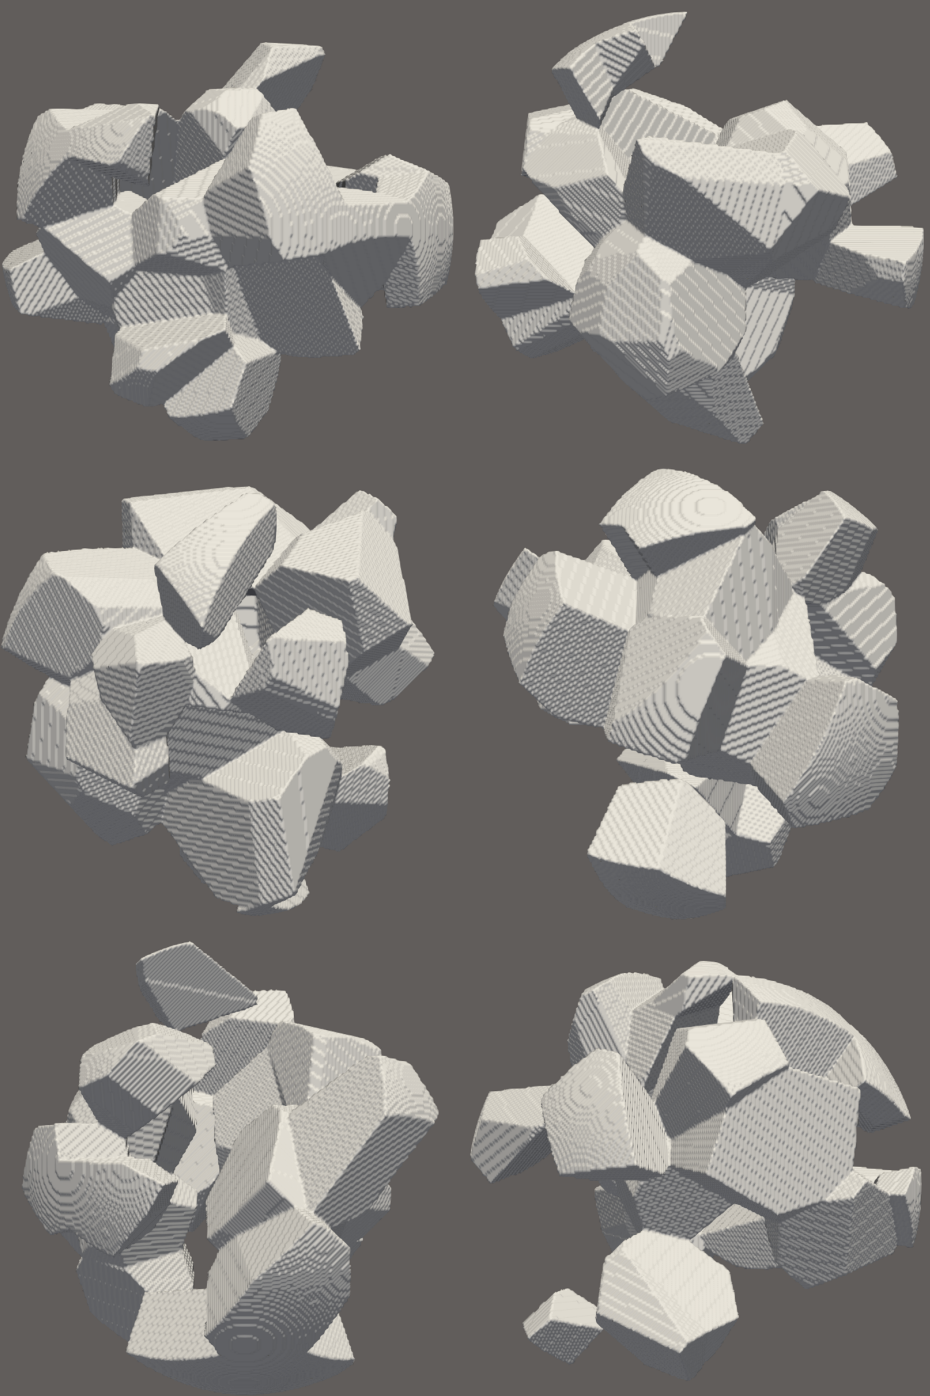
\includegraphics[width=0.3\textwidth]{../IMAGES/WRITEUP/NOTMINE/glitterinFigure1.png}
  \caption{Example of six irregular particles from \texttt{glitterin}. Figure from \cite{glitterin}. \note{ask for permission} }
  \label{fig: glitterin_dust_grains}
\end{figure*}



\question{As far as I know, glitterin is using $\omega$ and not $\omega_{eff}$, meaning when I present the results for spherical vs irregular, I'm comparing $P\omega_{eff}$ vs $P\omega$. I am not entirely sure how to get the $g$ factor I need to calculate $\omega_{eff}$ with gitterin. I only switched to $\omega_{eff}$ because of \cite{Zhang2023}. Should I switch the spherical back to just $\omega$ so they are comparing the same thing?}

\question{How much detail do I go into about glitterin?}